Im Folgenden werden Mockups präsentiert, welche das Design und die Benutzeroberfläche der PONG App darstellen. Kleinere Änderungen an Design und der Benutzeroberfläche während des Entwicklungsprozesses sind möglich.

\subsubsection{Icon Legende}
\vspace*{0.5cm}

\begin{center}
    \begin{tabular}{ll}
        
\includegraphics[width=1.5em,height=1.5em]{diagramme/assets/Media-Play-256.png} & Start / Fortsetzen \\
        
\includegraphics[width=1.5em,height=1.5em]{diagramme/assets/Media-Pause-256.png} & Pause \\
        
\includegraphics[width=1.5em,height=1.5em]{diagramme/assets/Close-256.png} & Beenden\\
        
\includegraphics[width=1.5em,height=1.5em]{diagramme/assets/Arrow-Left-05-256.png} & Zurück \\
        
\includegraphics[width=1.5em,height=1.5em]{diagramme/assets/Floppy-256.png} & Speichern und Fortfahren \\
        
\includegraphics[width=1.5em,height=1.5em]{diagramme/assets/Money-Coin-02-WF-256.png} & Coins / Kontostand \\
        
\includegraphics[width=1.5em,height=1.5em]{diagramme/assets/Heart-256.png} & Symbolisiert ein Leben \\
        
\includegraphics[width=1.5em,height=1.5em]{diagramme/assets/Globe-256.png} & Sprachauswahl \\
        
\includegraphics[width=1.5em,height=1.5em]{diagramme/assets/Shirt-256.png} & Allgemeines Symbol für Skins \\
        
\includegraphics[width=1.5em,height=1.5em]{diagramme/assets/list.png} & Top-10 Liste \\
        
\includegraphics[width=1.5em,height=1.5em]{diagramme/assets/Trophy-256.png} & Achivements \\
        
\includegraphics[width=1.5em,height=1.5em]{diagramme/assets/Bomb-256.png} & Beispiel für Powerup \\    
        
\includegraphics[width=1.5em,height=1.5em]{diagramme/assets/Lock-256.png} & Item gesperrt / nicht im Besitz
    \end{tabular}
\end{center}
\setlength{\extrarowheight}{0.5em}

\clearpage

\subsubsection{Dialog u00 - Hauptmenü}


\begin{wrapfigure}{l}{0.5\textwidth}
    \begin{center}
    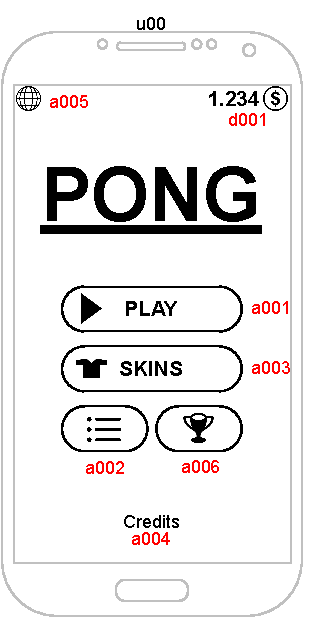
\includegraphics{diagramme/pdf/Mockup-u00.pdf}
    \end{center}
    \caption{Dialog u00 - Hauptmenü}
\end{wrapfigure}

Das Hauptmenü dient dem \gls{spieler} als Ausgangspunkt. Von hier aus kann es möglich sein die Sprache zu ändern (a005) und die persönlichen Achivements einzusehen (a006). 
Es muss hingegen möglich sein, die Anzahl der Coins einzusehen (d001), zur Spielauswahl zu gelangen (a001), zum InGame Store zu gelangen (a003), die TopTen Liste einzusehen (a002) und die Credits  zu öffnen (a004).

\clearpage

\subsubsection{Dialog u01 - Spielmodus Einstellungen}

\begin{wrapfigure}{l}{0.5\textwidth}
    \begin{center}
    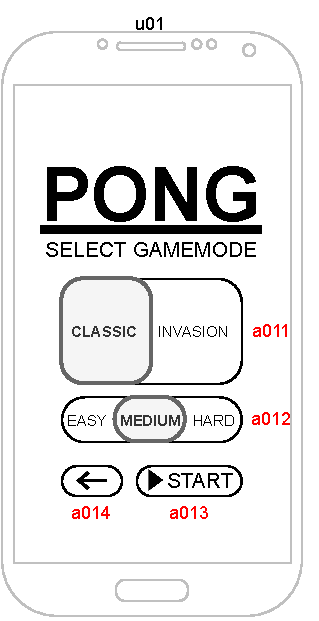
\includegraphics{diagramme/pdf/Mockup-u01.pdf}
    \end{center}
    \caption{Dialog u01 - Spielmodus Einstellungen}
\end{wrapfigure}

Möchte der \gls{spieler} ein Spiel starten, so kann er zunächst zwischen den Spielmodi "Classic" und "Invasion" wählen (a012). Der \gls{spieler} muss die Möglichkeit haben, von einem aus drei Schwierigkeitsstufen zu wählen (a011).
Außerdem muss es dem \gls{spieler} möglich sein, zurück zum Hauptmenü zu kommen (a015).
\clearpage

\subsubsection{Dialog u02a - Spiel Classic}

\begin{wrapfigure}{l}{0.5\textwidth}
    \begin{center}
    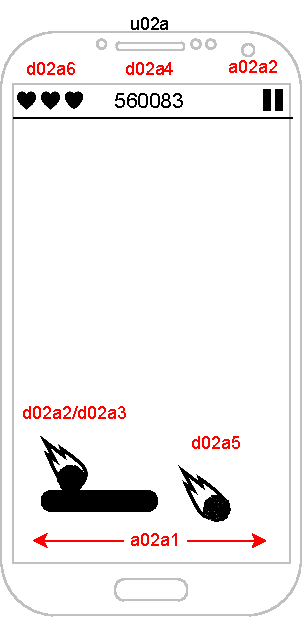
\includegraphics{diagramme/pdf/Mockup-u02a.pdf}
\end{center}
    \caption{Dialog u02a - Spiel Classic}
\end{wrapfigure}

Der Screen "Spiel Classic" muss neben dem beweglichen \gls{balken} (a02a1) und dem \gls{ball} die aktuelle Lebensanzeige und die aktuelle Punktzahl anzeigen.
Außerdem muss in der rechten oberen Ecke ein Pause-Button die möglichkeit bieten das aktuelle Spiel zu pausieren (a02a2).
Verpasst der Spieler den Ball mit dem Balken und der Ball berührt den unteren Bildschirmrand, so ist das Spiel verloren (d02a5).
\vspace*{1cm}
\clearpage

\subsubsection{Dialog u02b - Spiel Invasion}

\begin{wrapfigure}{l}{0.5\textwidth}
    \begin{center}
    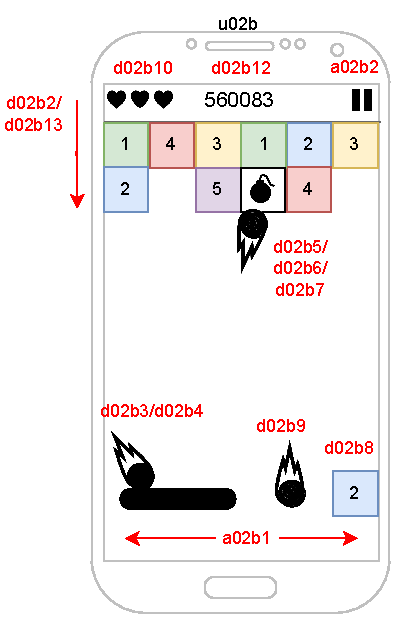
\includegraphics{diagramme/pdf/Mockup-u02b.pdf}
\end{center}
    \caption{Dialog u02b - Spiel Invasion}
\end{wrapfigure}

Bei dem optionalen Spielmodus "Invasion" können neben den UI Elementen aus u02a noch die Spielmodus spezifischen Elemente auftauchen. 
Hierbei handelt es sich um Blöcke, welche zerstört werden können. Hierbei können die Blöcke unterschiedliche Stärken besitzen. 
Die Stärke repräsentiert hierbei die Anzahl an \gls{ball}berührungen, die es benötigt um einen Block zu zerstören. Außerdem können Power-Up Blöcke
erscheinen, welche dem \gls{spieler} temporäre Vorteile verschaffen. Berührt rin Block den unteren Rand des Bildschirms, so ist das Spiel ebenfalls beendet (d02b8).
\clearpage

\subsubsection{Dialog u09 - Sprachauswahl}

\begin{wrapfigure}{l}{0.5\textwidth}
    \begin{center}
    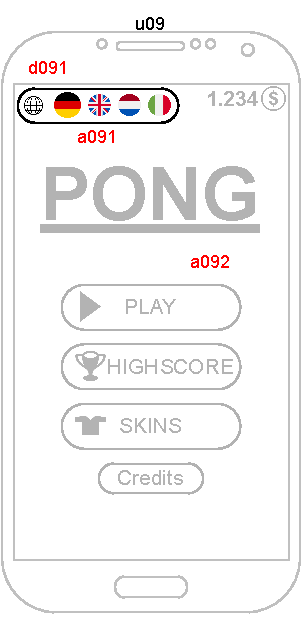
\includegraphics{diagramme/pdf/Mockup-u09.pdf}
\end{center}
    \caption{Dialog u09 - Sprachauswahl}
\end{wrapfigure}

Bei der optionalen Sprachauswahl kann der \gls{spieler} zwischen verschiedenen Sprachen wählen und somit den im Spiel angezeigten Text entsperchend der Auswahl ünersetzen lassen.
\clearpage

\subsubsection{Dialog u10 - Pause Menü}

\begin{wrapfigure}{l}{0.5\textwidth}
    \begin{center}
    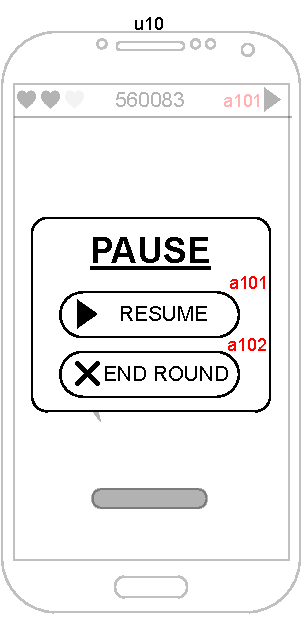
\includegraphics{diagramme/pdf/Mockup-u10.pdf}
\end{center}
    \caption{Dialog u10 - Pause Menü}
\end{wrapfigure}

Das Pause-Menü muss dem \gls{spieler} die Optionen geben, entweder das Spiel zu beenden (a102), oder das Spiel fortzusetzen (a101).

\clearpage

\subsubsection{Dialog u11 - Game-Over-Menü}

\begin{wrapfigure}{l}{0.5\textwidth}
    \begin{center}
    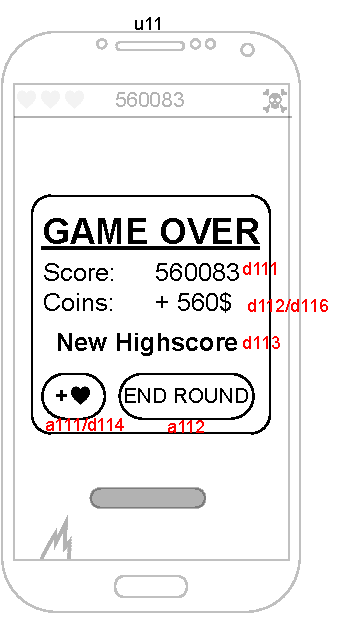
\includegraphics{diagramme/pdf/Mockup-u11.pdf}
    \end{center}
    \caption{Dialog u11 - Game-Over-Menü}
\end{wrapfigure}

Hat der \gls{spieler} keine Herzen mehr, so muss der Game-Over Screen angezeigt werden. Dieser bietet beim ersten Mal nach jeder Spielrunde die Möglichkeit ein letzte Chance zu bekommen (a111).
Außerdem muss der erreichte Score (d111) und die erspielten Coins (d112) angezeigt werden.
Der \gls{spieler} muss mit einem Klick auf "End Round" (a112) zurück ins Hauptmenü geleitet werden.
\clearpage

\subsubsection{Dialog u12 - Werbung}

\begin{wrapfigure}{l}{0.5\textwidth}
    \begin{center}
    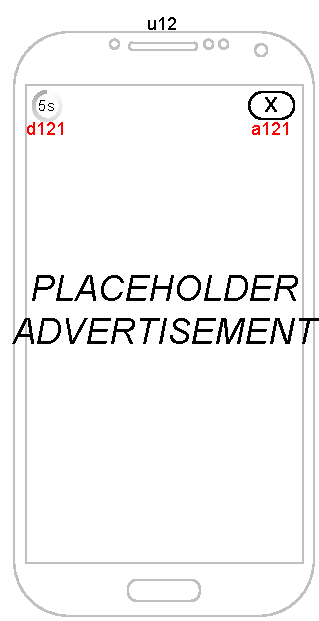
\includegraphics{diagramme/pdf/Mockup-u12.pdf}
    \end{center}
    \caption{Dialog u12 - Werbung}
\end{wrapfigure}

Entscheidet sich der \gls{spieler} dazu, ein weiteres Leben durch einen Werbeclip zu bekommen, so muss eine Platzhalter-Werbung angezeigt werden.
Nach Ablauf der Werbung, muss der \gls{spieler} diese beenden (a121) und kann weiter spielen.
\clearpage

\subsubsection{Dialog u13 - Namenseingabe}

\begin{wrapfigure}{l}{0.5\textwidth}
    \begin{center}
    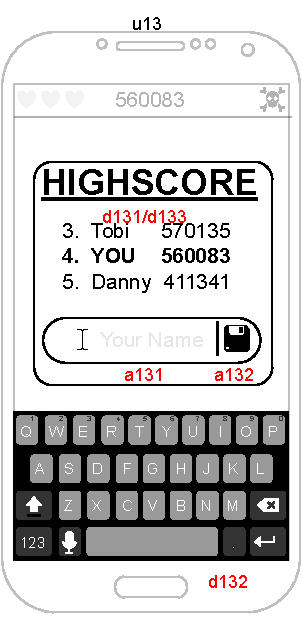
\includegraphics{diagramme/pdf/Mockup-u13.pdf}
\end{center}
    \caption{Dialog u13 - Namenseingabe}
\end{wrapfigure}

Hat der \gls{spieler} eine TopTen Platzierung erspielt, so muss ihm seine Position in der TopTen Liste nach Ablauf der Spielrunde angezeigt werden.
Neben dem gerade erspieleten Score müssen ebenfalls die zwei nächsten Scores angezeigt werden.
Der \gls{spieler} muss dann die Möglichkeit haben, seinen Namen einzutragen (a131) und sich mit einem Klick auf den Speichern Button (a132) in der TopTen Liste abzuspeichern.
\clearpage

\subsubsection{Dialog u20 - Top-10 Liste}

\begin{wrapfigure}{l}{0.5\textwidth}
    \begin{center}
    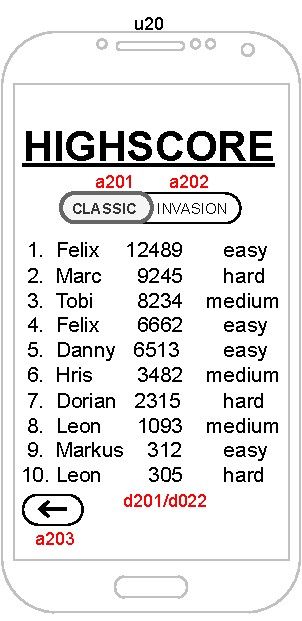
\includegraphics{diagramme/pdf/Mockup-u20.pdf}
\end{center}
    \caption{Dialog u20 - Top-10 Liste}
\end{wrapfigure}

Die TopTen Liste muss die zehn besten Scores präsentieren und es kann für jeden Spielmodus eine einzelne Liste geben. 
Neben der Platzierung, dem Namen und der Punkte, muss ebenfalls der Spielmodus angezeigt werden, mit welchem die Platzierung erreicht wurde.
\clearpage

\subsubsection{Dialog u25 - Achivements}

\begin{figure}[h!]
    \begin{center}
        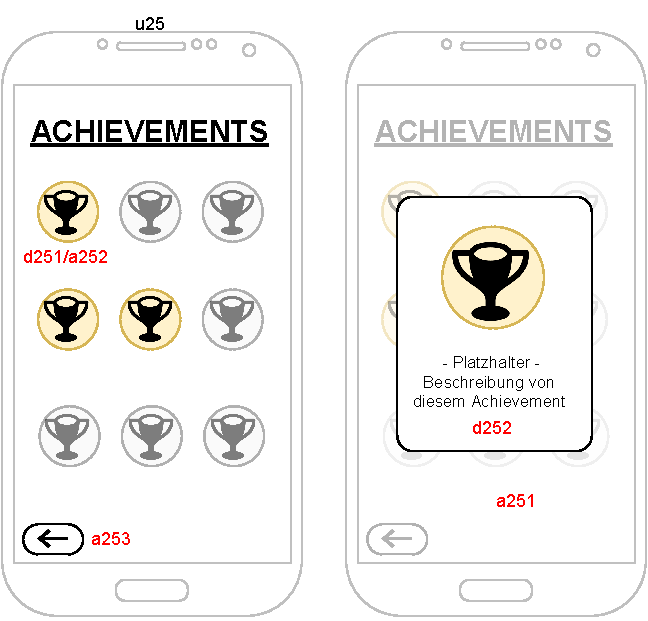
\includegraphics{diagramme/pdf/Mockup-u25.pdf}
    \end{center}
    \caption{Dialog u25 - Achivements}
\end{figure}

Auf dem Achivements Bildschirm sollen alle erreichbaren \gls{achievements} als Symbol dargestellt werden. Noch nicht freigeschaltete \gls{achievements} sollen  ausgegraut dargestellt werden. Klickt der \gls{spieler} auf ein Achivementsymbol, soll die dazugehörige Beschreibung angezeugt werden. Ein Klick außerhalb der Beschreibung soll diese wieder schließen. Dem \gls{spieler} soll es möglich sein, durch einen Klick auf den Zurück-Pfeil wieder ins Hauptmenü zu gelangen.
\clearpage

\subsubsection{Dialog u30 - Skin Auswahl}

\begin{wrapfigure}{l}{0.5\textwidth}
    \begin{center}
    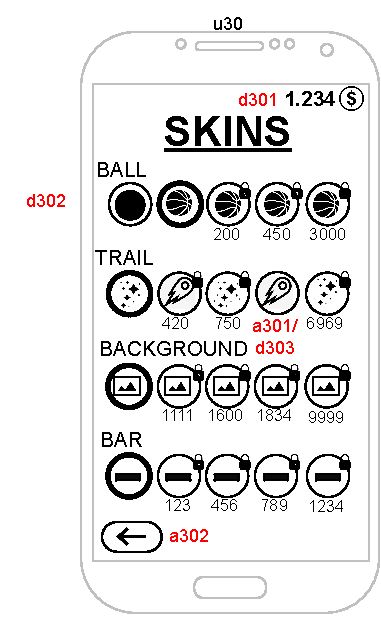
\includegraphics{diagramme/pdf/Mockup-u30.pdf}
\end{center}
    \caption{Dialog u30 - Skin Auswahl}
\end{wrapfigure}

Die Skin-Auswahl bietet dem \gls{spieler} fünf Skins, jeweils für den \gls{ball}, den Schweif, den Hintergrund und der Bar an.
Dem \gls{spieler} muss es möglich sein, durch einen Klick auf den Zurück-Pfeil wieder ins Hauptmenü zu gelangen.
\clearpage

\subsubsection{Dialog u31 - Skin Kauf}

\begin{wrapfigure}{l}{0.5\textwidth}
    \begin{center}
    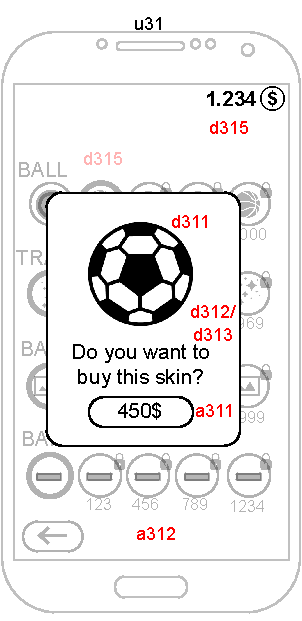
\includegraphics{diagramme/pdf/Mockup-u31.pdf}
\end{center}
    \caption{Dialog u31 - Skin Kauf}
\end{wrapfigure}

Kauft der \gls{spieler} einen Skin, so muss der Skin vergrößert angezeigt werden. Außerdem muss der Preis angezeigt werden.
\clearpage

\subsubsection{Dialog u40 - Credits}

\begin{wrapfigure}{l}{0.5\textwidth}
    \begin{center}
    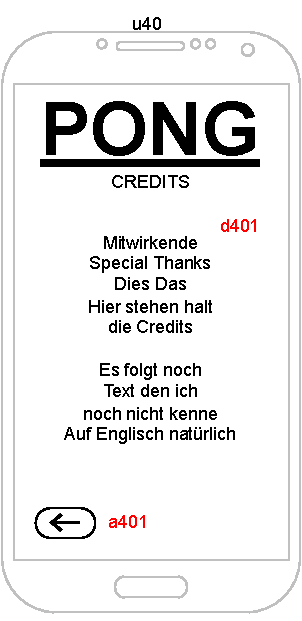
\includegraphics{diagramme/pdf/Mockup-u40.pdf}
    \caption{Dialog u40 - Credits}
    \end{center}
\end{wrapfigure}

Der \gls{spieler} muss die Möglichkeit haben in den Credits genauere Informationen zum Entwicklerteam, und zur App allgemein zu bekommen.
Durch einen Klick auf den zurück-Pfeil, muss der Nutzer wieder ins Hauptmenü gelangen.
\clearpage